\section{Data Collection Study}

\begin{margintable}
	\vspace{-4.73cm}
	\centering
	\begin{tabularx}{1\marginparwidth}{XXd{2.2}d{2.2}d{2.2}}
		
		\toprule
		
		\textbf{Model}&\textbf{Phone}&\multicolumn{1}{c}{\textbf{0ms}}&\multicolumn{1}{c}{\textbf{33ms}}&\multicolumn{1}{c}{\textbf{66ms}} \\
		\midrule
		
		\multirow{8}{*}{\textsc{single}}   &\multirow{2}{*}{\textbf{S3}}  &12.50&13.17&14.40       \\
		&                              &(7.36)&(7.82)&(8.24)       \\
		\cmidrule(r){2-5}		
		&\multirow{2}{*}{\textbf{S4}}  &17.25&18.77&19.41       \\
		&                              &(9.94)&(10.76)&(10.78)       \\
		\cmidrule(r){2-5}						 				   
		&\multirow{2}{*}{\textbf{N5X}} &17.01&18.09&19.96       \\
		&                              &(9.76)&(10.39)&(10.93)       \\
		\cmidrule(r){2-5}										   
		&\multirow{2}{*}{\textbf{N6}}  &18.87&19.78&21.52       \\
		&                              &(11.4)&(12.15)&(12.7)       \\	
		
		\midrule
		
		\multirow{8}{*}{\textsc{general}} &\multirow{2}{*}{\textbf{S3}}   &12.95&13.48&14.52        \\
		&                               &(7.57)&(7.92)&(8.38)        \\ 
		\cmidrule(r){2-5}
		&\multirow{2}{*}{\textbf{S4}}   &16.79&17.69&18.70        \\
		&                               &(10.61)&(10.99)&(11.21)        \\
		\cmidrule(r){2-5}
		&\multirow{2}{*}{\textbf{N5X}}  &17.39&18.02&19.46	        \\
		&                               &(10.61)&(10.88)&(11.60)        \\
		\cmidrule(r){2-5}									      
		&\multirow{2}{*}{\textbf{N6}}   &17.53&17.75&19.53        \\ 
		&                               &(11.59)&(11.94)&(12.72)       \\									         		
		\bottomrule    
	\end{tabularx}%
	\caption[Model results]{\small Average test euclidean distances (mm) and standard deviations (brackets) for single and general models for all configurations.}
	\label{tab:results}
\end{margintable}

We conducted a data collection study to gather IMU data while performing touches on a smartphone.
Our collected data set consists of 6 smartphone sensors that were sampled while participants performed successive touches on the smartphones front side. 
For our data collection study we used a repeated-measures design with one independent variable: \textsc{phone}, which was counterbalanced using Latin Balanced squares. 
The total amount of conditions was: \textsc{phone} $ = 4$.

\subsection{Apparatus}
Our dataset was generated using four different sized smartphones on which participants had to perform a certain amount of touches (for further information see \cref{sec:tasks}).
The phones we used were a Samsung S3 Mini, a Samsung S4, a Google Nexus 5X, and a Motorola Nexus 6.
For more details about the devices used in the study see \cref{tab:devices}.
Our used phone sizes range from $ 4^{\prime\prime} $ (S3) to $ 6^{\prime\prime} $ (N6). 
Using phones of these sizes we were able to cover the sizes of everyday smartphones, including some high-end devices and create a generalizable machine-learning model.



\subsection{Tasks}
\label{sec:tasks}

%\begin{marginfigure}
%	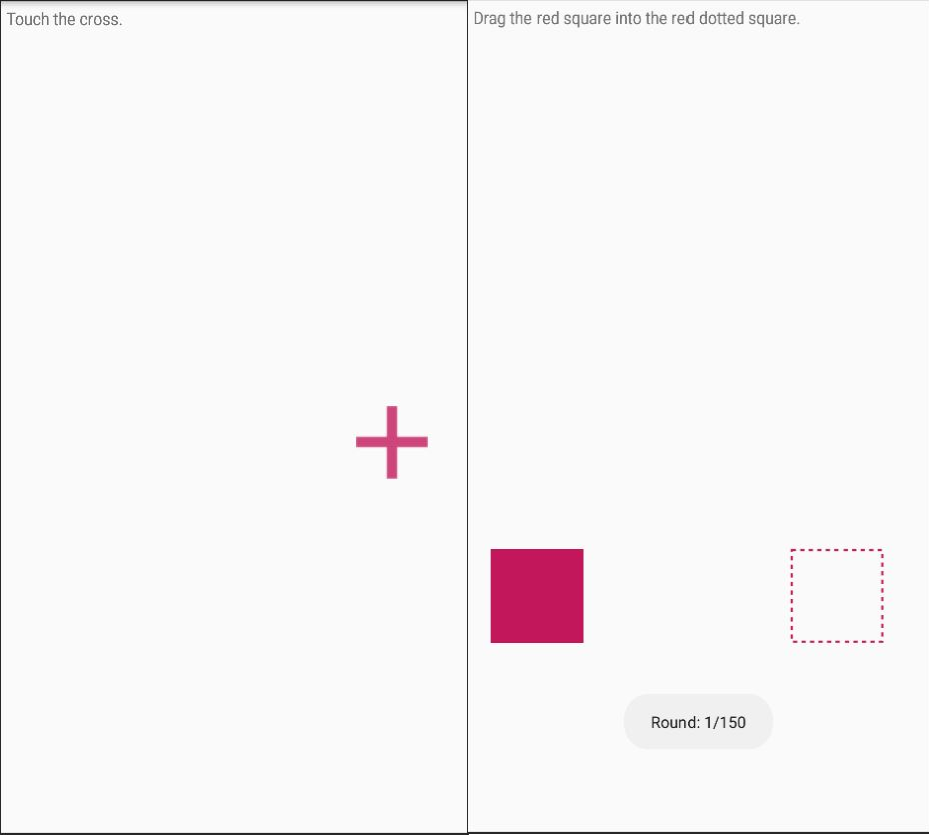
\includegraphics[width=\marginparwidth]{scur}
%	\caption{SCUR.}
%	\label{fig:tasks}
%\end{marginfigure}



For our data collection study participants had to touch points displayed as crosses in a 16 $ \times $ 9 grid on the touchscreen (see \cref{fig:touchtask}). 
%We aligned the touch points displayed as crosses in a 16 $ \times $ 9 grid. 
To achieve a high variance, we randomized the positions of the crosses within all the cells.
To avoid sequential effects, we randomized the order in which the crosses were displayed.
There were a total of 3 repetitions, resulting in a total  of $ 16 \times 9 \times 3 = 432 $ touches on one device.

Between two touches our study participants had to perform a simple \textit{Fitts' Law task} (see \cref{fig:fittstask}). 
Here participants had to drag a filled rectangle into a dashed contour of a rectangle.
This task was mainly implemented to reset the participants grip to the bottom half of the device.
Because a previous shifted grip of the hand to the upper half of the phone influences the recorded sensor data when reaching for the next target in the lower half and vice versa.
\subsection{Procedure}
Participants were either invited within the course \textit{FIS'18} or orally.
All appointments were discussed orally.
After participants have arrived they signed a consent form, and we continued measuring their hand length.
We asked the participants to take a seat on a chair without armrests and explained the study procedure and its sense.
We started carrying out the study and handed out the first phone accordingly to the balanced Latin Square order. 
After participants finished the tasks (see \cref{sec:tasks}) on the first phone, we asked them if they need a short recovery break and then continued with the next phones.
Additionally, we allowed participants to rest and put away the phone during the \textit{Fitt's Law task} because we specifically deal with this task in our preprocessing step (see \cref{sec:prepro}).
The study duration was 54 minutes on average.

\subsection{Participants}
%Some sentences are copied from Beens BA, is this sufficient? ASK SVEN OR HUY
We invited 20 right-handed fellow students as participants (15 male, 5 female).
Their age ranged between 21 and 27 ($ M=24.25$ , $SD=1.58 $). 
We measured the hand length of participants. 
The size was measured from the tip of the middle finger to the wrist crease with fingers stretched out.
Hand lengths ranged from $16.0cm$ to $21.3cm$ ($M=19.3cm$ , $SD=1.47cm$).
Our measured data covers samples from the 5th and 95th percentile of the anthropometric data reported in previous work \cite{Poston}.  
